\documentclass[main.tex]{subfiles}

\begin{document}

\subsection{Secondo esercizio}
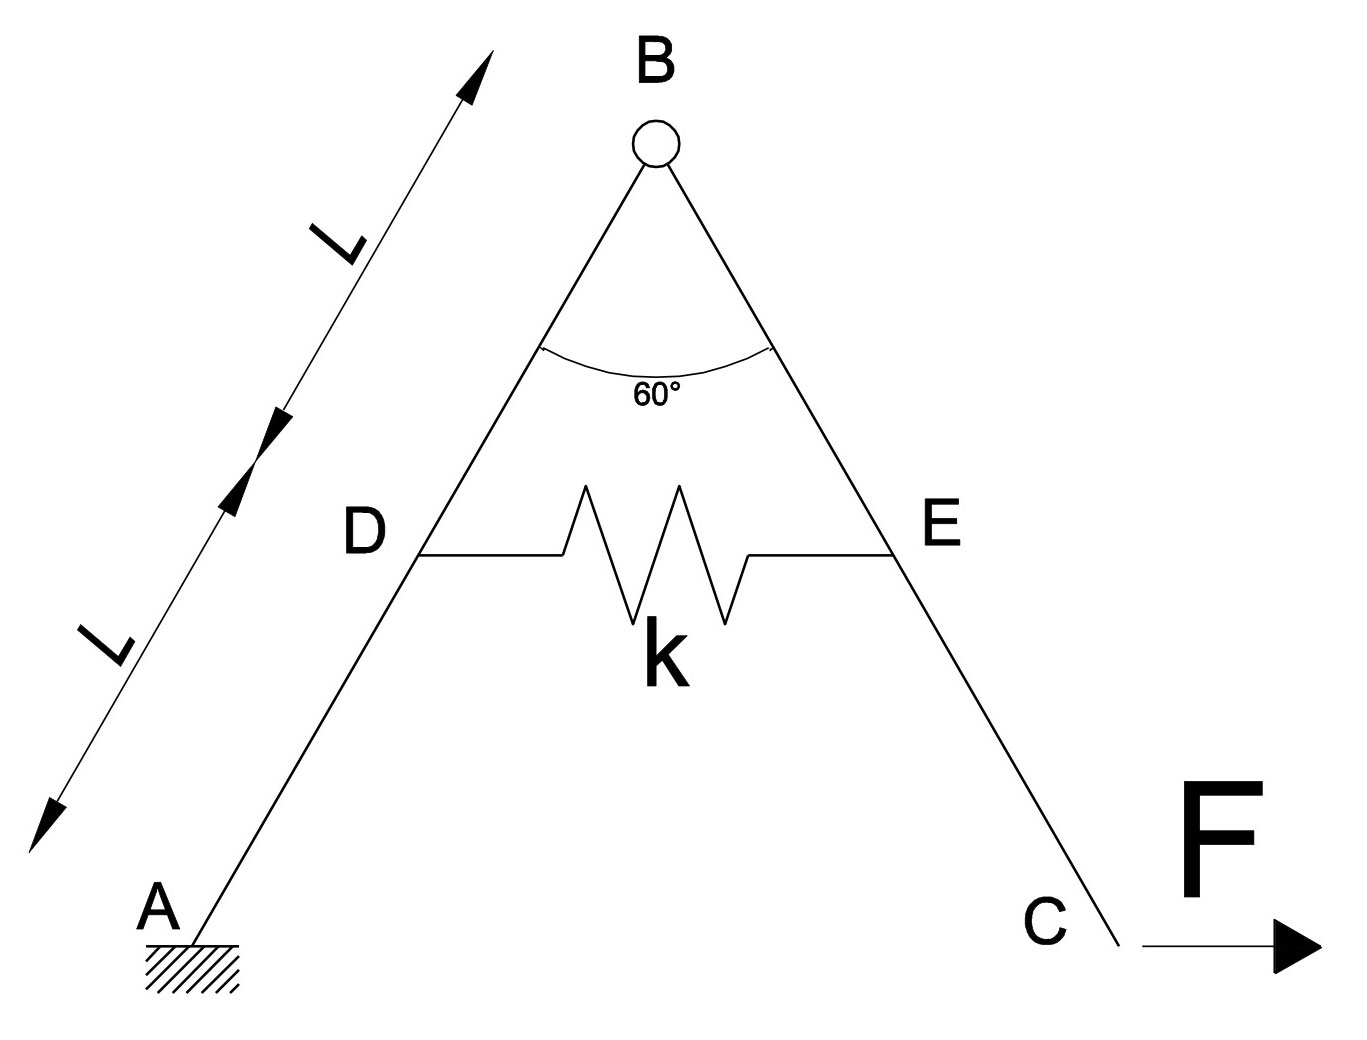
\includegraphics[width=\textwidth]{2015-0109-2.jpg}

Nel sistema rappresentato in figura una molla di rigidezza incognita collega i punti medi delle due aste AB e BC. Una forza $F$, nota, è applicata in direzione orizzontale nel punto C. Si chiede di:

\begin{enumerate}
\item Calcolare la rigidezza k della molla affinché il sistema in figura sia nella posizione di equilibrio (si consideri pari $\dfrac{L}{2}$ la lunghezza $L_0$ della molla indeformata);
\item Disegnare i diagrammi delle azioni interne nell’asta AB.
\end{enumerate}

\clearpage

\subsection{Soluzione secondo esercizio}

\subsubsection{Osservazioni}

\begin{enumerate}
\item La struttura è formata da due aste, un vincolo a incastro, un vincolo a cerniera e la molla, che si comporta come una biella trasmettendo l'azione assiale.
\item La struttura è identificabile come un triangolo equilatero, per l'angolo  a $\dfrac{\pi}{3}$ in B.
\end{enumerate}

\subsubsection{Analisi dei vincoli}
Tramite il computo dei gradi di vincolo possiamo fare una verifica preliminare si isostaticità:

\begin{figure}[H]
  \begin{subfigure}[b]{.5\textwidth}
  \centering
  \[
  	gdv: \begin{cases}
		gdv_{molla} = 1\\
		gdv_{incastro} = 3\\
		gdv_{cerniera} = 2(2-1) = 2
  	\end{cases}
  \]
  \caption{Gradi di vincolo del sistema.}
  \end{subfigure}
  \hfill
  \begin{subfigure}[b]{.5\textwidth}
  \centering
  \[
  	gdl: \begin{cases}
  		gdl_{aste} = 6\\
  	\end{cases}  
  \]
  \caption{Gradi di libertà del sistema.}
  \end{subfigure}
  \caption{Verifica preliminare di isostaticità.}
\end{figure}

Per la verifica preliminare, la struttura risulta isostatica.

\subsubsection{Primo punto}

\paragraph{Analisi dei vincoli esterni}
L'unico vincolo a terra è l'incastro nel punto A:

\begin{figure}[H]
\centering
\resizebox{.5\textwidth}{!}{% First image 2015 06 29

\begin{tikzpicture}

  \tiny


  \point{c}{0}{0}
  \point{c1}{0}{0.8}
  \point{c2}{-0.8}{0}
  \point{a}{2-1.41421}{1.41421}
  \point{a1}{2-1.41421}{0.8+1.41421}
  \point{d}{2}{0}
  \point{b}{2+1.41421}{-1.41421}
  \point{b1}{2+1.41421}{-1.41421-1.3}

  \beam{2}{c}{d}[0][1];
  \beam{2}{a}{b};

  \load{1}{a}[180][0.5]
  \load{1}{a1}[270][0.5]

  \load{2}{c}
  \load{1}{c}[180][0.5]
  \load{1}{c}[270][0.5]

  \load{1}{b1}[90][1]

  \notation{1}{c}{$\vec{M}_C$}[below right]
  \notation{1}{c}{$\vec{H}_C$}[below left]
  \notation{1}{c}{$\vec{V}_C$}[above right]

  \notation{1}{a}{$\vec{H}_A$}[below left]
  \notation{1}{a}{$\vec{V}_A$}[above right]

  \notation{1}{b}{$\vec{F}$}[below right]

  % \notation{1}{a1}{$\vec{H}_A$}
  % % \notation{1}{d1}{$\vec{R}_D$}
  % % \notation{1}{b1}{$\vec{H}_B$}[below left]
  % \notation{1}{c1}{$\vec{F}$}[above left]

  %  % \support{3}{o};

  %  % %Degrees
  %  % \notation{1}{o}{$\alpha$}[above];
  %  % \notation{1}{a}{$\beta$}[above];

  %  % \notation{5}{o}{a}[$a$];
  %  % \notation{5}{a}{b}[$b$];
  %  % \notation{5}{o}{b}[$c$];

\end{tikzpicture}}
\caption{Reazioni vincolari dei vincoli esterni}
\end{figure}

\[
\begin{cases}
	F - H_A = 0 \\
	V_A = 0 \\
	M_A = 0	
\end{cases}
\Longrightarrow
\begin{cases}
	H_A = F \\
	V_A = 0 \\
	M_A = 0	
\end{cases}
\]

\paragraph{Analisi delle reazioni vincolari nell'asta AB}

\begin{figure}[H]
\centering
\resizebox{.5\textwidth}{!}{% First image 2015 06 29

\begin{tikzpicture}

  \tiny

  \point{a}{0}{0}
  \point{c}{1}{0}
  \point{b}{2}{2}
  \point{d}{1}{1}

  \beam{2}{a}{b}

  \load{1}{b}[180][0.5]
  \load{1}{a}[180][0.5]
  \load{1}{a}[90][1]

  \load{1}{d}[0][1]
  \load{1}{d}[-90][1]

  \notation{1}{a}{$\vec{F}$}[below left]
  \notation{1}{a}{$2\vec{F}$}[above left]

  \notation{1}{b}{$\vec{F}$}[above left]

  \notation{1}{d}{$\vec{R}_{D_x}$}[below right]
  \notation{1}{d}{$\vec{R}_{D_y}$}[below left]

\end{tikzpicture}}
\caption{Reazioni vincolari nell'asta AB}
\end{figure}

\[
\begin{cases}
	H_A + R_D + H_B = 0\\
	LR_{t_D}	- 2LH_{t_B} = 0\\
	R_{t_D} = R_D*\sin\left(-\dfrac{\pi}{6} \right)\\
	H_{t_B}= H_B*\sin\left(\pi - \dfrac{\pi}{6} \right)
\end{cases}
\Longrightarrow
\begin{cases}
	F + R_D + H_B = 0\\
	LR_{t_D}	- 2LH_{t_B} = 0\\
	R_{t_D} = -\dfrac{\sqrt{3}}{2}R_D\\
	H_{t_B}= \dfrac{\sqrt{3}}{2}H_B\\
\end{cases}
\Longrightarrow
\begin{cases}
	F + R_D + H_B = 0\\
	R_{t_D} = 2H_{t_B}\\
	R_D = -\dfrac{2}{\sqrt{3}}R_{t_D} = -2H_B \\
	H_B = \dfrac{2}{\sqrt{3}}H_{t_B} = \dfrac{R_{t_D}}{\sqrt{3}}\\
\end{cases}
\]

\[
\begin{cases}
	F -2H_B + H_B = 0\\
	R_{t_D} = 2H_{t_B}\\
	R_D = -\dfrac{2}{\sqrt{3}}R_{t_D} = -2H_B \\
	H_B = \dfrac{2}{\sqrt{3}}H_{t_B} = \dfrac{R_{t_D}}{\sqrt{3}}\\
\end{cases}
\Longrightarrow
\begin{cases}
	H_B = F \\
	R_{t_D} = 2H_{t_B}\\
	R_D = -2F\\
	H_B = 2H_{t_B} = R_{t_D}\\
\end{cases}
\]

Sapendo che la formula della forza elastica è:

\begin{figure}[H]
	\[
		F_{el} = -k\Delta L
	\]
	\caption{Formula forza elastica}
\end{figure}

E che la lunghezza corrente della molla è di $L$, possiamo calcolare il delta come $\Delta L = L - \dfrac{L}{2} = \dfrac{L}{2}$

\begin{equation}
	-2F = -k\Delta L
\end{equation}

\begin{equation}
	2f = k\dfrac{L}{2}
\end{equation}

\begin{equation}
	k = \dfrac{4F}{L}
\end{equation}

\subsubsection{punto}
Separo le componenti dei 3 vettori, in \textit{sforzo normale} e \textit{taglio}:

\paragraph{Sforzo normale}

\[
	N = \dfrac{F}{2}
\]

Nella parte inferiore la scomposizione dei vettori $H_A$ e $R_D$ danno luogo ad una trazione, per cui lo sforzo è positivo, mentre nella parte superiore si ha una contrazione, per cui lo sforzo è negativo.

\begin{figure}[H]
\centering
\resizebox{.3\textwidth}{!}{\begin{tikzpicture}

  \tiny

  \point{a}{0}{0};
  \point{b}{1}{0};
  \point{c}{2}{0};

  \beam{2}{a}{c}

  \internalforces{a}{b}{-0.25}{-0.25};
  \internalforces{b}{c}{0.25}{0.25}[0][blue];


\end{tikzpicture}}
\caption{Grafico sforzo normale nell'asta AB}
\end{figure}

\paragraph{Taglio}

\[
	T = \dfrac{\sqrt{3}F}{2}
\]

Nella parte inferiore la scomposizione dei vettori $H_A$ e $R_D$ danno luogo ad una rotazione oraria, per cui il taglio è positivo, mentre nella parte superiore si ha una rotazione antioraria, per cui il taglio è negativo.

\begin{figure}[H]
\centering
\resizebox{.3\textwidth}{!}{% First image 2015 06 29

\begin{tikzpicture}

  \tiny

  \point{a}{0}{0}
  \point{e}{2.5}{-0.866}
  \point{b}{0.5}{0.866}
  \point{d}{1.5}{0.866}
  \point{c}{1}{2*0.866}

  \beam{2}{a}{c}

  \internalforces{a}{b}{0.866}{0.866}[0][blue];
  \internalforces{b}{c}{-1.732}{-1.732}[0][red];

\end{tikzpicture}}
\caption{Grafico taglio nell'asta AB}
\end{figure}

\paragraph{Momento flettente}

\[
	M_{max} = L\dfrac{\sqrt{3}F}{2}
\]

Il momento aumenta linearmente fino a raggiungere il massimo nel punto D, in cui la forza $R_D$ viene applicata, che impone un momento negativo e porta a decrescere linearmente il momento flettente sino a raggiungere 0 nell'estremo opposto.

\begin{figure}[H]
\centering
\resizebox{.3\textwidth}{!}{% First image 2015 06 29

\begin{tikzpicture}

  \tiny

  \point{h}{-1.2}{0};
  \point{a}{0}{0};
  \point{b}{1}{0};
  \point{c}{2}{0};

  \beam{2}{a}{c}


  \notation{1}{a}{A}[above];
  \notation{1}{b}{B}[above];
  \notation{1}{c}{C}[above];

  %  \notation{1}{b}{B}[above left];
  %  \notation{1}{c}{C}[above=0.1];
  %  \notation{1}{d}{D}[above right];
  %  \notation{1}{e}{E}[above right];
  %  \notation{1}{f}{$\vec{F}$}[above right];

  %  %Degrees
  %  \notation{1}{a}{$\frac{\pi}{3}$}[above right=0.325];
  %  \notation{1}{e}{$\frac{\pi}{3}$}[above left=0.325];

  \internalforces{a}{b}{1}{1}[0][red];
  \internalforces{b}{c}{1}{0}[0][red];

\end{tikzpicture}}
\caption{Grafico momento flettente nell'asta AB}
\end{figure}

\end{document}